\documentclass[tikz,border=0pt]{standalone}

\usepackage[T1]{fontenc}
\usepackage{newtxtext,newtxmath}
\usepackage{graphicx}
\usetikzlibrary{calc,arrows.meta}
\hyphenpenalty=10000
\exhyphenpenalty=10000

% Visual styles for the three-column workflow figure.
\definecolor{workflowPanel}{HTML}{F0F0F0}
\definecolor{workflowText}{HTML}{111111}
\definecolor{workflowMuted}{HTML}{4B4B4B}
\definecolor{workflowGrid}{HTML}{B7B7B7}
\definecolor{workflowSand}{HTML}{EE945B}
\definecolor{workflowClay}{HTML}{432B1E}
\definecolor{workflowBlue}{HTML}{1769AA}
\definecolor{workflowFault}{HTML}{A7ADB4}
\definecolor{workflowCyan}{HTML}{35A6B4}
\definecolor{workflowOrange}{HTML}{E09200}
\definecolor{workflowYellow}{HTML}{F1C72D}
\definecolor{workflowOverburden}{HTML}{C6B06E}
\definecolor{workflowTopSeal}{HTML}{5F382D}
\definecolor{workflowStorageReservoir}{HTML}{D59B47}
\definecolor{workflowUnderburden}{HTML}{A8B3BF}

% PNAS research articles use 9 pt body text. Keep all figure-authored text at
% that same final-size scale; hierarchy comes from weight and placement.
\newcommand{\workflowtextsize}{\fontsize{9}{10.4}\selectfont}

\tikzset{
  workflow panel title/.style={
    inner sep=0pt,
    text=workflowText,
    font=\fontsize{10.5}{12}\selectfont,
    align=center,
  },
  workflow column title/.style={
    inner sep=0pt,
    text=workflowText,
    font=\workflowtextsize\bfseries,
    align=center,
  },
  workflow left title/.style={
    inner sep=0pt,
    text=workflowText,
    font=\workflowtextsize,
    align=center,
  },
  workflow heading/.style={
    anchor=west,
    inner sep=0pt,
    text=workflowText,
    font=\workflowtextsize\bfseries,
  },
  workflow left heading/.style={
    anchor=west,
    inner sep=0pt,
    text=workflowText,
    font=\workflowtextsize,
  },
  workflow body/.style={
    anchor=north west,
    inner sep=0pt,
    text=workflowText,
    align=left,
    font=\workflowtextsize,
  },
  workflow small/.style={
    anchor=north west,
    inner sep=0pt,
    text=workflowMuted,
    align=left,
    font=\workflowtextsize,
  },
  workflow figure label/.style={
    inner sep=0pt,
    text=workflowText,
    font=\workflowtextsize,
    align=center,
  },
  workflow schematic label/.style={
    inner sep=0pt,
    text=workflowText,
    font=\fontsize{8}{9.2}\selectfont,
    align=center,
  },
  workflow legend label/.style={
    anchor=west,
    inner sep=0pt,
    text=workflowText,
    font=\workflowtextsize,
    align=left,
  },
  workflow asset/.style={inner sep=0pt},
}

\newcommand{\workflowlegendbox}[4]{%
  \fill[#3] (#1,#2) rectangle ++(1.7,1.7);%
  \draw[workflowText,line width=0.25pt] (#1,#2) rectangle ++(1.7,1.7);%
  \node[workflow legend label] at (#1+2.5,#2+0.85) {#4};%
}

\newcommand{\workflowasset}[5]{%
  \node[workflow asset] at (#1,#2) {%
    \includegraphics[width=#3,height=#4,keepaspectratio]{#5}%
  };%
}

\newcommand{\workflowbullet}[4]{%
  \fill[workflowText] (#1,#2) rectangle ++(1.05,1.05);%
  \node[workflow heading,text width=#3] at (#1+2.3,#2+0.55) {#4};%
}

\newcommand{\workflowleftbullet}[4]{%
  \fill[workflowText] (#1,#2) rectangle ++(1.05,1.05);%
  \node[workflow left heading,text width=#3] at (#1+2.3,#2+0.55) {#4};%
}

\newcommand{\workflowsubbullet}[4]{%
  \fill[workflowText] (#1,#2) circle[radius=0.42mm];%
  \node[workflow body,text width=#3] at (#1+1.8,#2+0.35) {#4};%
}

\newcommand{\workflowopenbullet}[4]{%
  \draw[workflowText,line width=0.35pt] (#1,#2) circle[radius=0.55mm];%
  \node[workflow body,text width=#3] at (#1+1.8,#2+0.35) {#4};%
}


\begin{document}
\begin{tikzpicture}[x=1mm,y=1mm]
  % Preserve the reference composition and add a dedicated caption margin.
  \path[use as bounding box] (0,-12.5) rectangle (190,118.775);
  \fill[white] (0,-12.5) rectangle (190,118.775);

  % Column titles and light-gray workflow panels follow the reference layout.
  \node[workflow panel title] at (31.5,114.3) {Local fault property modeling};
  \node[workflow panel title] at (95.0,114.3) {Full-fault property sampling};
  \node[workflow panel title] at (158.5,114.3) {Field-scale CO$_2$ storage simulation};
  \draw[-{Stealth[length=1.8mm,width=1.2mm]},draw=workflowBlue!55!workflowMuted,line width=0.45pt]
    (60.0,114.3) -- (66.0,114.3);
  \draw[-{Stealth[length=1.8mm,width=1.2mm]},draw=workflowBlue!55!workflowMuted,line width=0.45pt]
    (121.0,114.3) -- (127.0,114.3);

  \path[fill=workflowPanel,rounded corners=2.4mm] (1.0,3.0) rectangle (62.0,109.0);
  \path[fill=workflowPanel,rounded corners=2.4mm] (64.5,3.0) rectangle (125.5,109.0);
  \path[fill=workflowPanel,rounded corners=2.4mm] (128.0,3.0) rectangle (189.0,109.0);

  % -----------------------------------------------------------------------
  % Column 1: local fault property modeling.
  % -----------------------------------------------------------------------
  \workflowleftbullet{15.2}{104.8}{38mm}{Geologic uncertainty}
  \node[workflow figure label] at (14.3,98.0) {%
    \shortstack[c]{A throw-window\\geologic model}%
  };
  \node[workflow body,anchor=center,text width=31.5mm] at (44.0,98.0) {%
    Vary structural and\\
    stratigraphic parameters
  };

  % Representative W4 stratigraphy for the medium-sand uniform scenario.
  % Both fault blocks contain horizontal S-C-S-C packages; the contacts are
  % offset across the dipping fault rather than connected by sloping layers.
  \begin{scope}[xshift=-1.6mm,yshift=1.8mm]
    % Footwall: four equal-thickness horizontal layers.
    \begin{scope}
      \clip (6.2,74.2) -- (6.2,91.2) -- (7.8,91.2) --
            (23.9,74.2) -- cycle;
      \fill[workflowSand] (6.2,74.2) rectangle (25.5,78.5);
      \fill[workflowClay] (6.2,78.5) rectangle (25.5,82.7);
      \fill[workflowSand] (6.2,82.7) rectangle (25.5,87.0);
      \fill[workflowClay] (6.2,87.0) rectangle (25.5,91.2);
      \draw[workflowText,line width=0.35pt] (6.2,78.5) -- (25.5,78.5);
      \draw[workflowText,line width=0.35pt] (6.2,82.7) -- (25.5,82.7);
      \draw[workflowText,line width=0.35pt] (6.2,87.0) -- (25.5,87.0);
    \end{scope}

    % Hanging wall: the same horizontal sequence shifted downward by throw.
    \begin{scope}
      \clip (7.8,91.2) -- (25.5,91.2) -- (25.5,74.2) --
            (23.9,74.2) -- cycle;
      \fill[workflowSand] (6.2,74.2) rectangle (25.5,76.7);
      \fill[workflowClay] (6.2,76.7) rectangle (25.5,80.7);
      \fill[workflowSand] (6.2,80.7) rectangle (25.5,84.7);
      \fill[workflowClay] (6.2,84.7) rectangle (25.5,91.2);
      \draw[workflowText,line width=0.35pt] (6.2,76.7) -- (25.5,76.7);
      \draw[workflowText,line width=0.35pt] (6.2,80.7) -- (25.5,80.7);
      \draw[workflowText,line width=0.35pt] (6.2,84.7) -- (25.5,84.7);
    \end{scope}

    \draw[workflowText,line width=0.45pt] (6.2,74.2) rectangle (25.5,91.2);
    \draw[workflowText,line width=1.0pt] (7.8,91.2) -- (23.9,74.2);
    \draw[white,line width=0.50pt] (7.8,91.2) -- (23.9,74.2);
    \draw[white,line width=0.45pt,->] (10.4,88.5) -- (12.8,88.5);
    \node[workflow schematic label,anchor=east,text=white] at (24.7,88.5) {Fault core};
    \node[workflow schematic label,anchor=west] at (7.3,76.2) {Sand};
    \node[workflow schematic label,anchor=west,text=white] at (7.3,80.5) {Clay};
  \end{scope}

  \node[workflow body] at (29.0,92.0) {%
    $\left.
      \begin{array}{@{}l@{}}
        z_f\\
        T_i\\
        V_{\mathrm{cl,sand}}\\
        V_{\mathrm{cl,clay}}
      \end{array}
    \right\}$%
  };
  \node[workflow figure label] at (50.5,84.5) {%
    \shortstack[c]{162 geologic\\scenarios}%
  };

  \workflowleftbullet{8.0}{70.0}{48mm}{Stochastic fault-core architectures}
  \node[workflow figure label] at (31.0,66.0) {$N=2{,}000$ per geologic scenario};
  \node[workflow figure label] at (9.5,62.1) {1};
  \node[workflow figure label] at (21.5,62.1) {2};
  \node[workflow figure label] at (50.5,62.1) {$N$};
  \node[workflow asset] at (9.5,54.0) {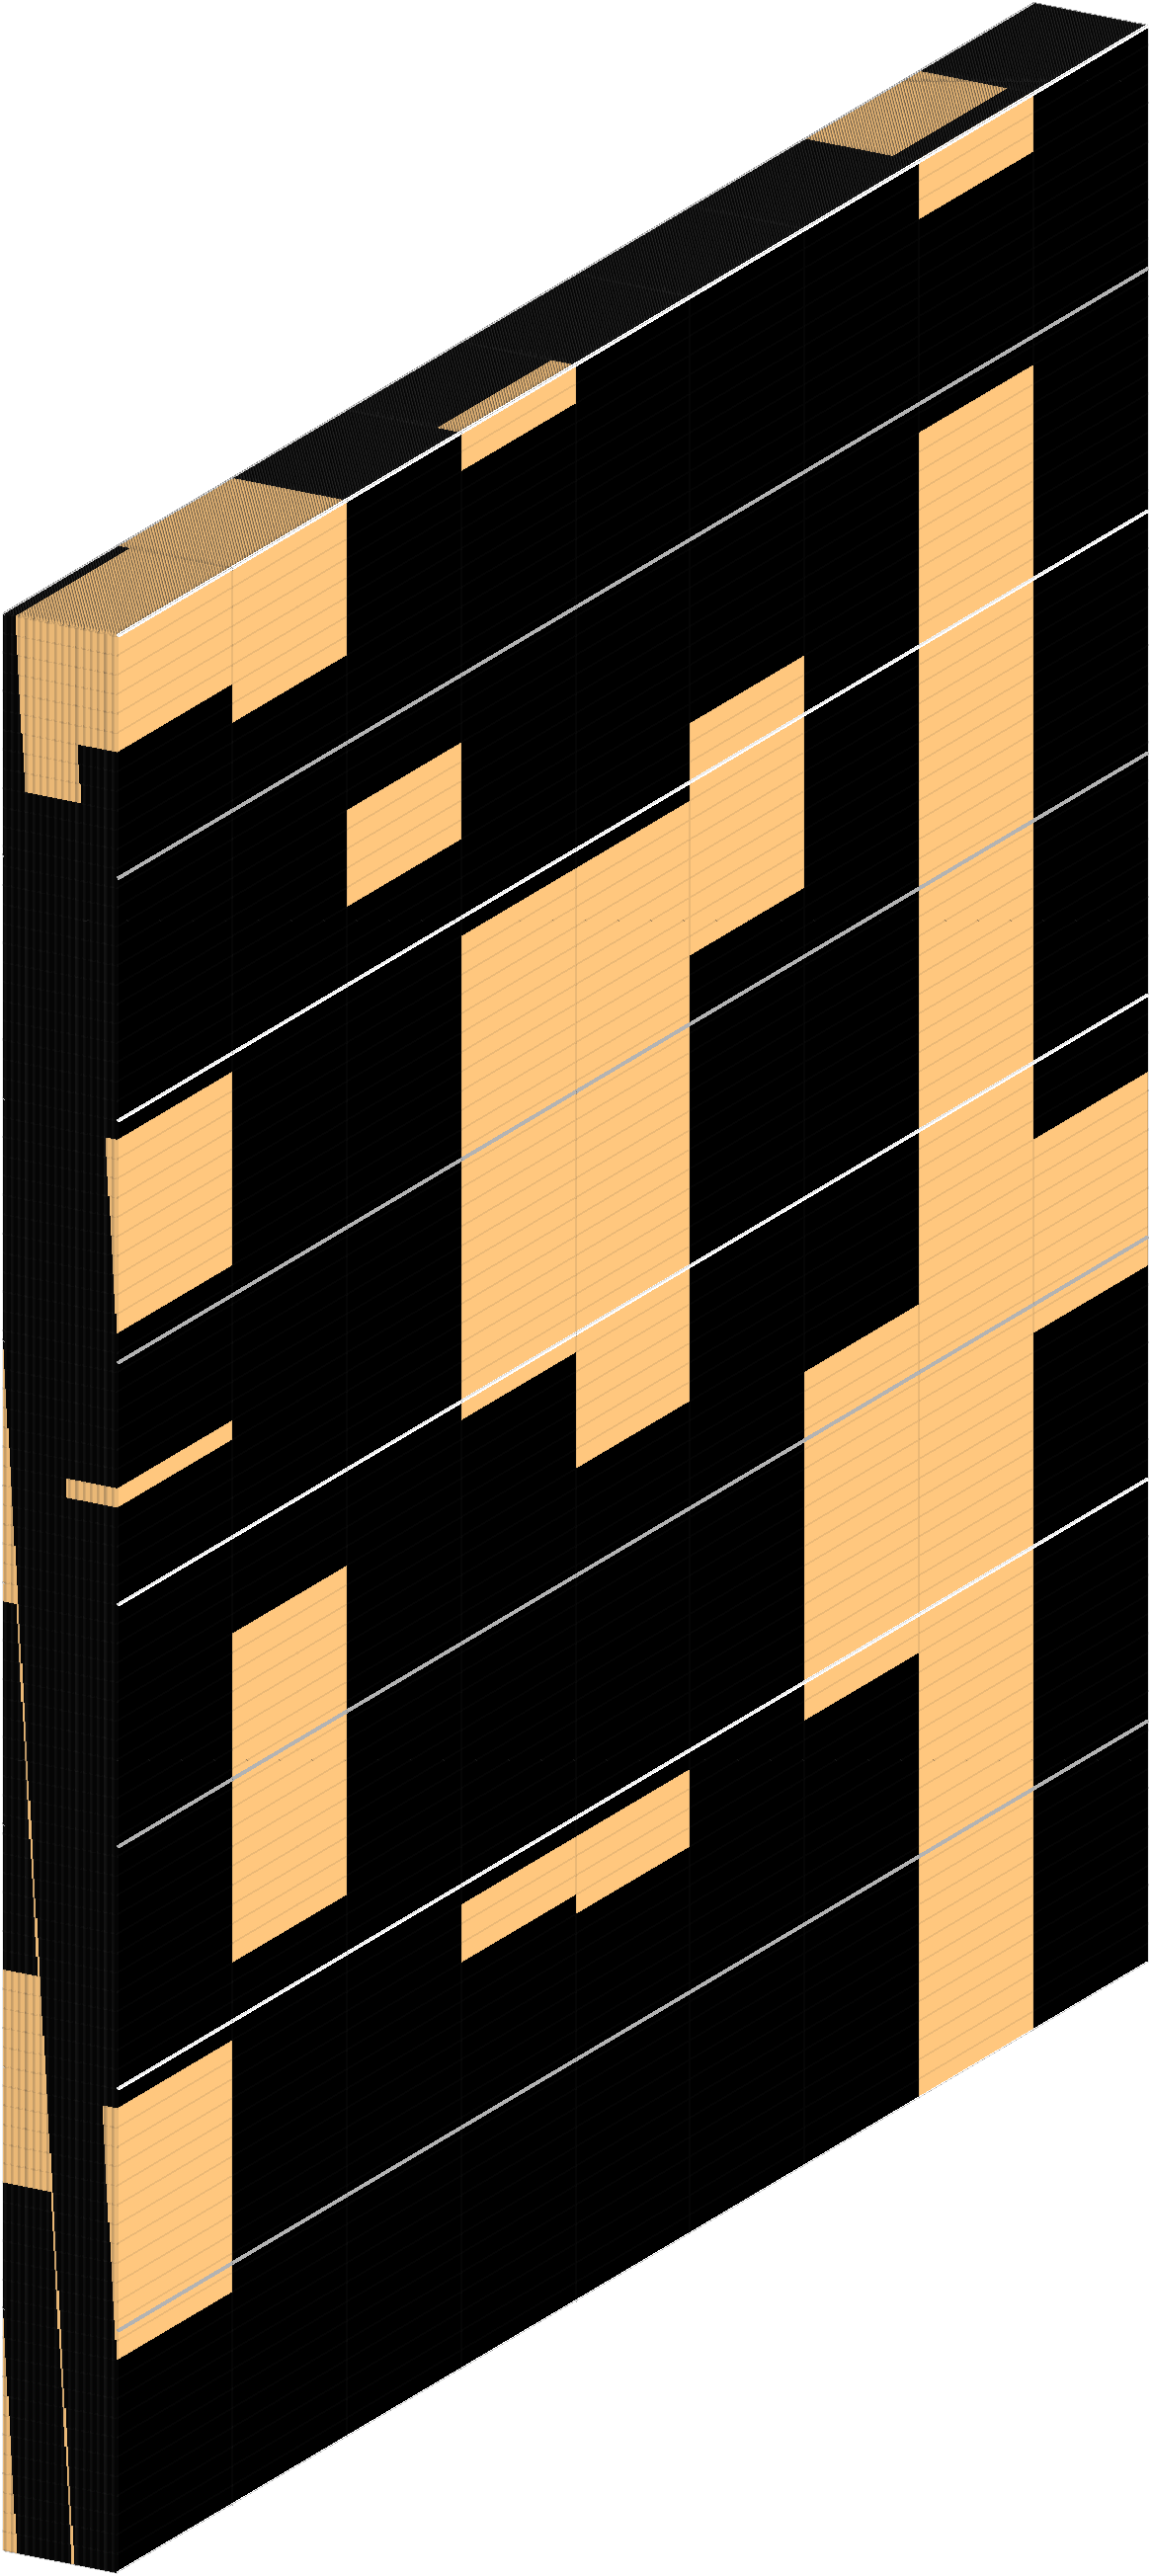
\includegraphics[width=9.2mm,height=13mm,keepaspectratio]{assets/derived/fault_architecture_01.png}};
  \node[workflow asset] at (21.5,54.0) {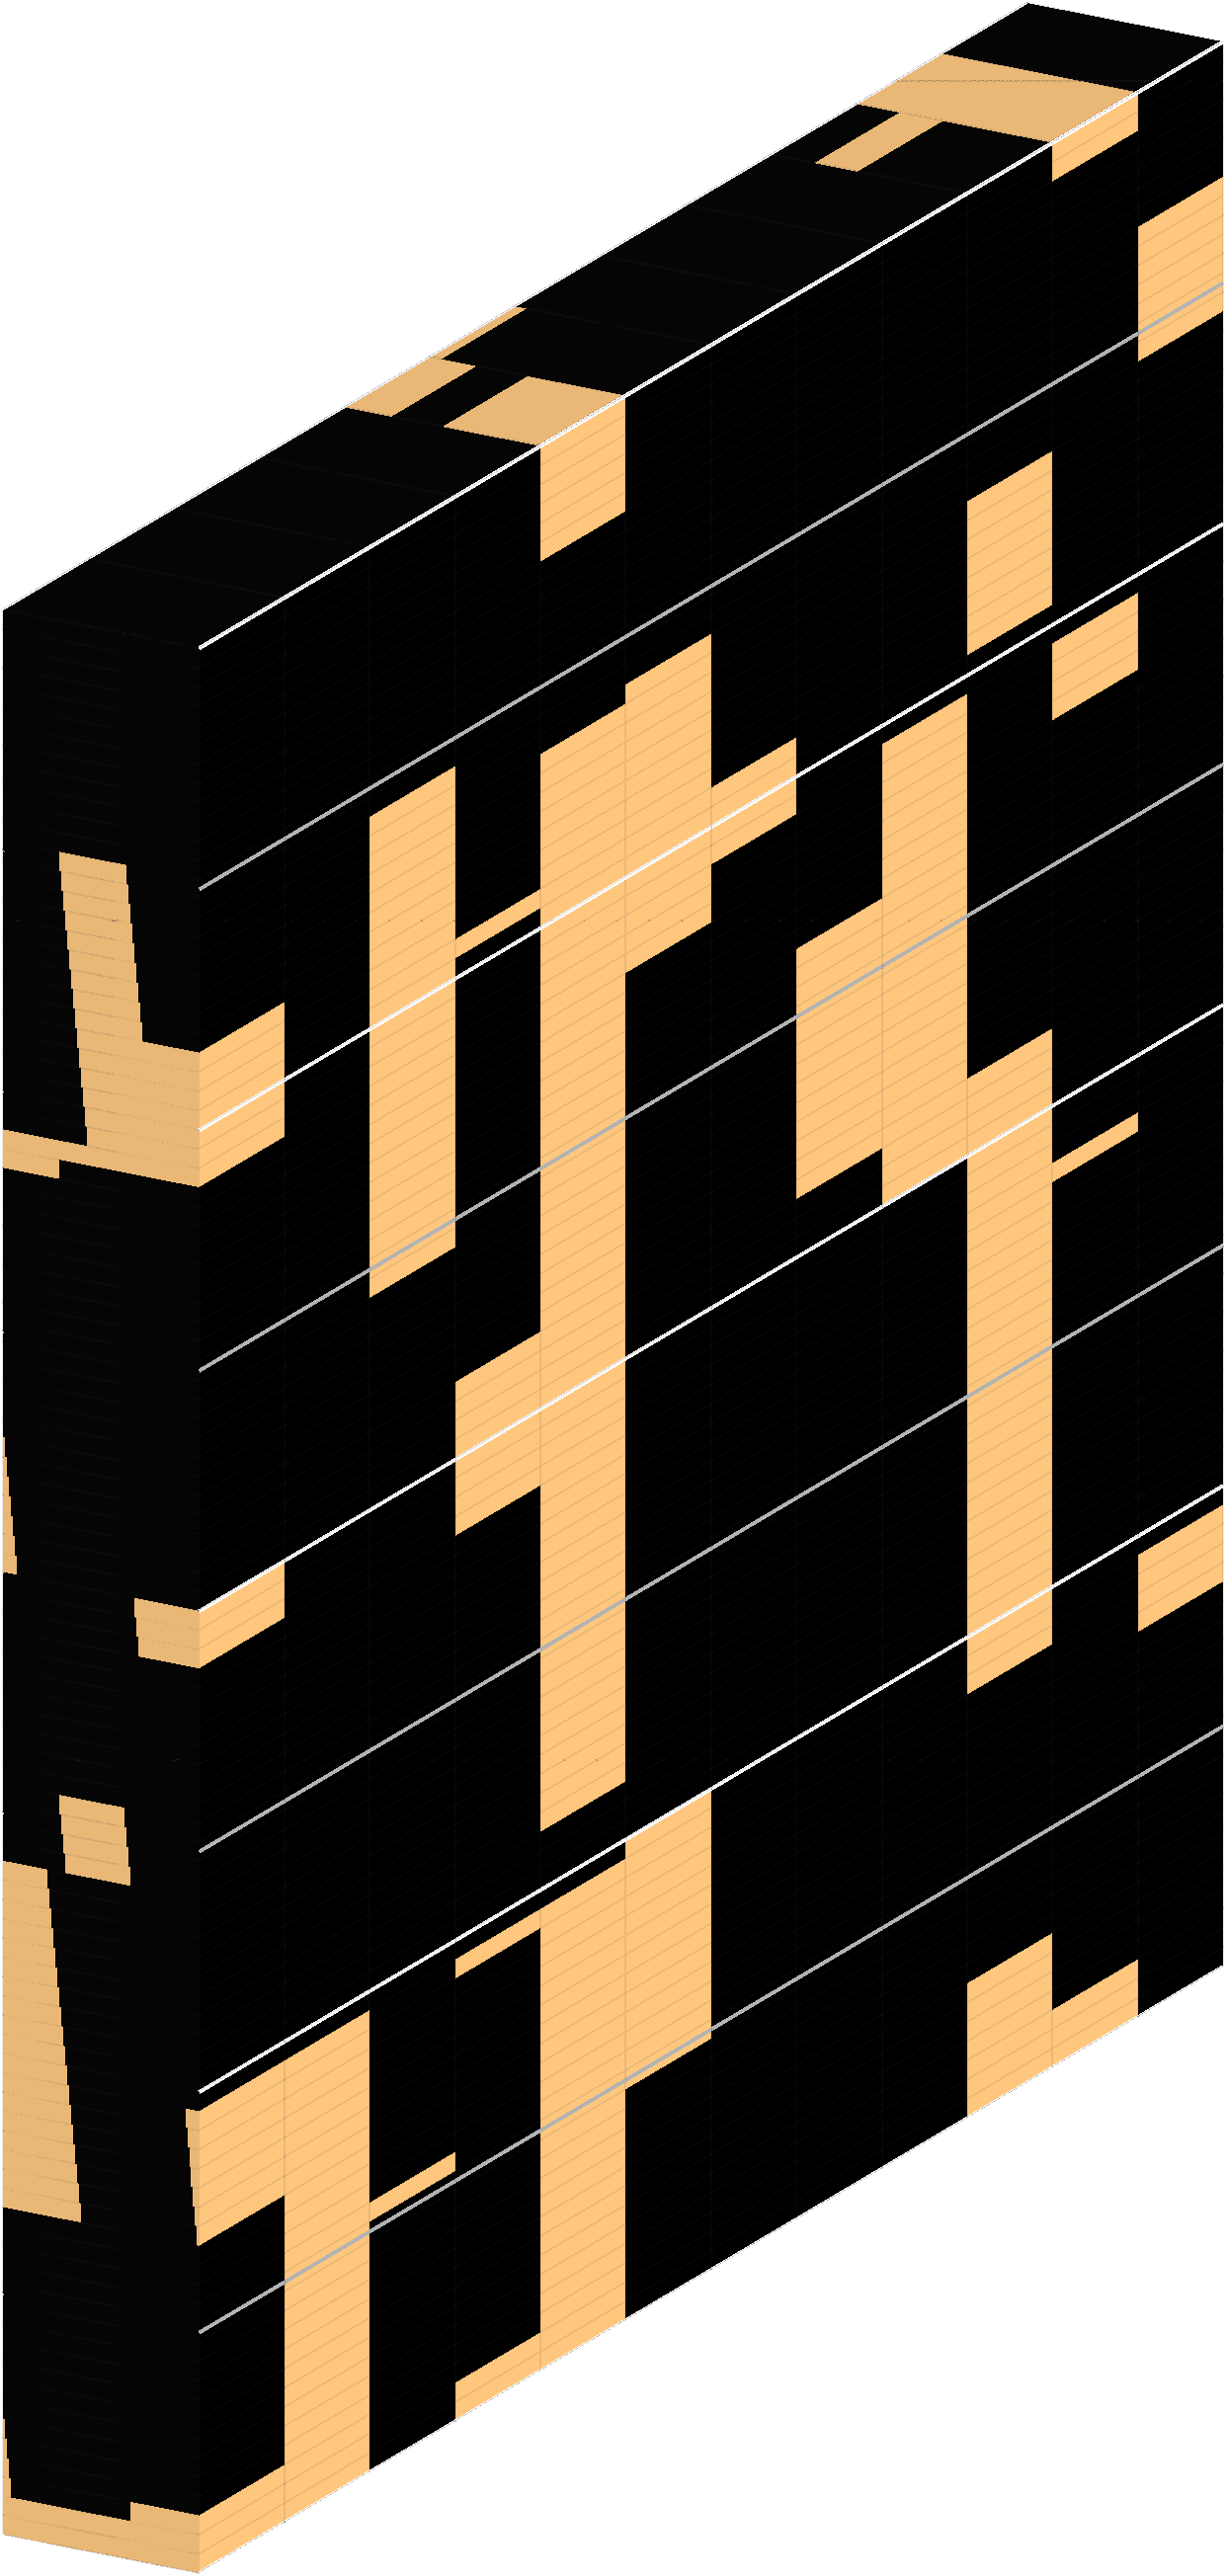
\includegraphics[width=9.2mm,height=13mm,keepaspectratio]{assets/derived/fault_architecture_02.png}};
  \node[workflow figure label] at (36.0,54.0) {$\cdots$};
  \node[workflow asset] at (50.5,54.0) {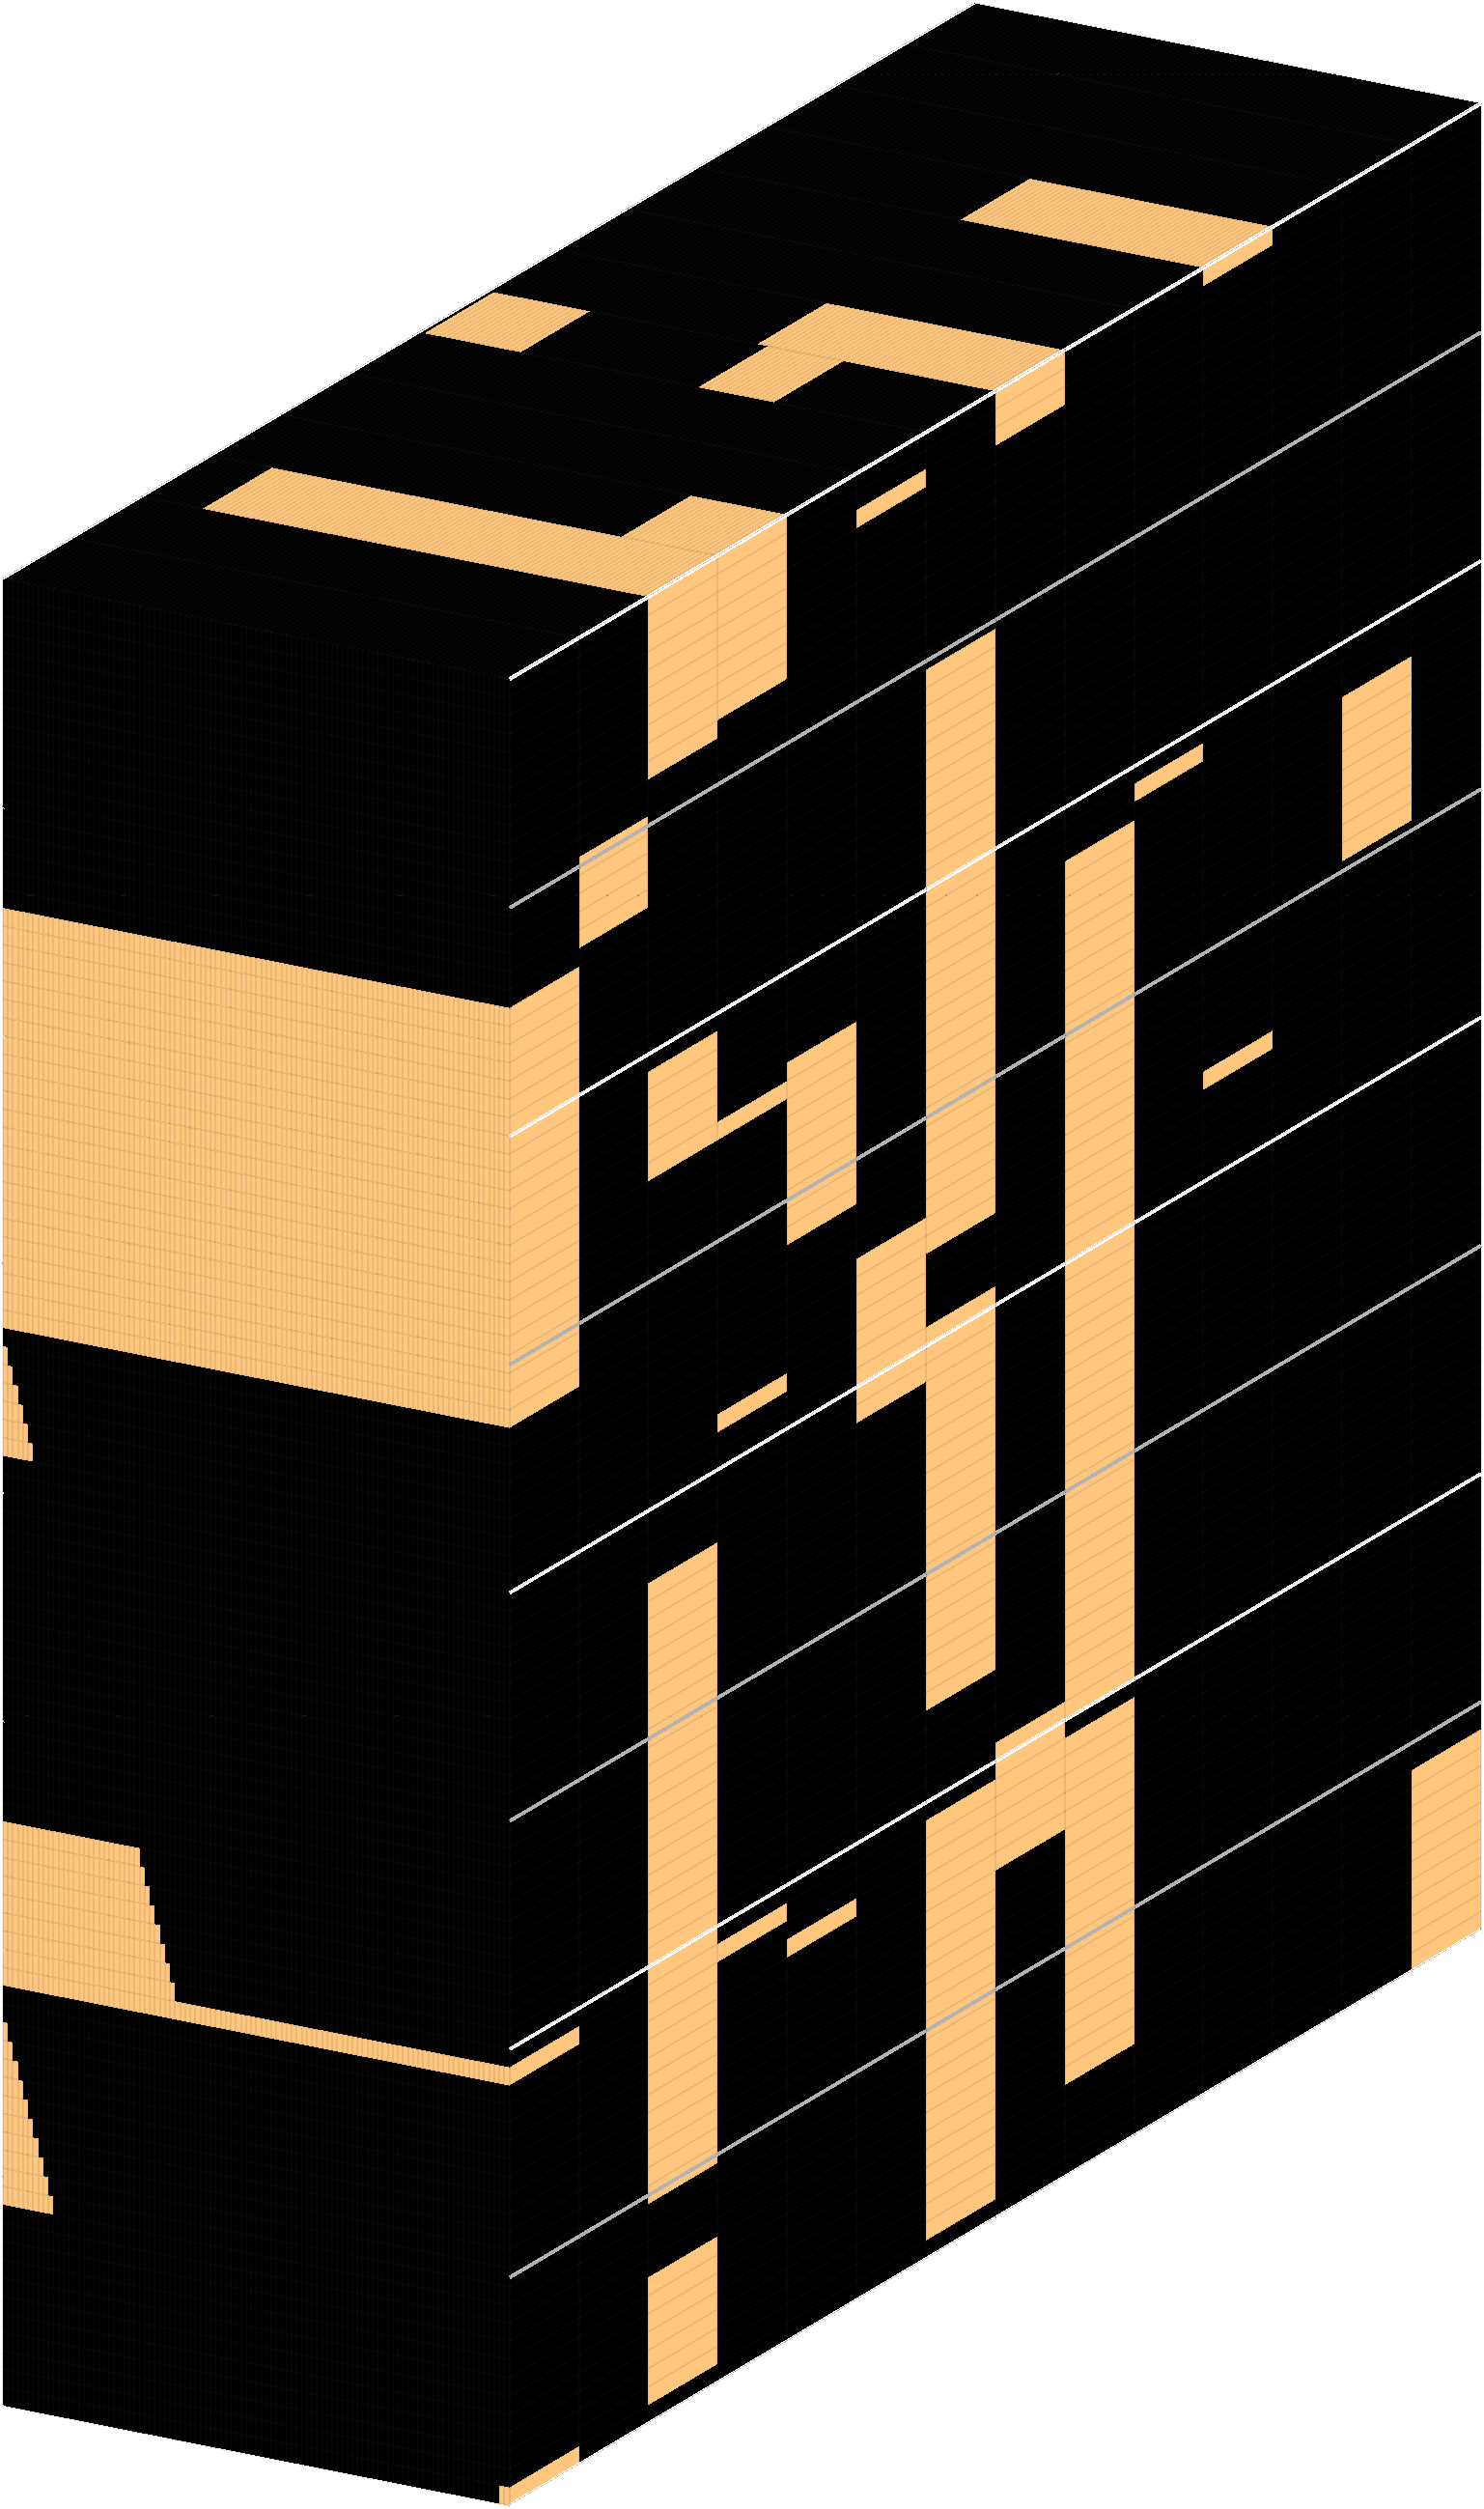
\includegraphics[width=9.2mm,height=13mm,keepaspectratio]{assets/derived/fault_architecture_04.png}};

  \workflowleftbullet{4.0}{42.0}{55mm}{Physics-based fault-property upscaling}
  \workflowasset{16.2}{21.2}{28mm}{35mm}{assets/derived/permeability_distributions.pdf}
  \workflowasset{47.0}{21.2}{28mm}{35mm}{assets/derived/pc_kr_curves.pdf}

  % -----------------------------------------------------------------------
  % Column 2: hierarchical full-fault sampling.
  % -----------------------------------------------------------------------
  \fill[workflowText] (80.8,104.8) rectangle ++(1.05,1.05);
  \node[workflow left title] at (95.0,105.35) {%
    3D fault geometry
  };

  % Actual field-scale fault geometry extracted from the simulation VTU.
  \workflowasset{95.0}{93.0}{46.5mm}{13.5mm}{assets/fault_geometry_3d.png}
  \node[workflow schematic label,anchor=east] at (88.0,101.0) {Strike};
  \draw[->,line width=0.45pt,workflowText]
    (88.7,101.0) -- (94.0,101.0);
  \node[workflow schematic label,anchor=east] at (75.2,92.7) {Dip};
  \draw[->,line width=0.45pt,workflowText]
    (76.1,94.7) -- (77.7,90.5);
  \node[workflow schematic label,text=white] at (95.0,92.2) {%
    Top-seal fault region
  };
  \node[workflow figure label] at (95.0,83.4) {%
    6 windows along dip $\times$ 87 slices along strike
  };

  \fill[workflowText] (75.7,78.25) rectangle ++(1.05,1.05);
  \node[workflow left title] at (95.0,78.8) {%
    Fault property realizations
  };
  \node[workflow figure label] at (95.0,74.2) {%
    Example $K$ and $\phi$ fields
  };

  \node[workflow figure label,anchor=east] at (73.2,69.8) {$K_{xx}$};
  \workflowasset{81.2}{69.8}{14.8mm}{3.4mm}{assets/derived/panel2_kxx_case01.pdf}
  \workflowasset{97.2}{69.8}{14.8mm}{3.4mm}{assets/derived/panel2_kxx_case03.pdf}
  \workflowasset{113.2}{69.8}{14.8mm}{3.4mm}{assets/derived/panel2_kxx_case07.pdf}
  \node[workflow figure label,anchor=east] at (73.2,65.05) {$K_{yy}$};
  \workflowasset{81.2}{65.05}{14.8mm}{3.4mm}{assets/derived/panel2_kyy_case01.pdf}
  \workflowasset{97.2}{65.05}{14.8mm}{3.4mm}{assets/derived/panel2_kyy_case03.pdf}
  \workflowasset{113.2}{65.05}{14.8mm}{3.4mm}{assets/derived/panel2_kyy_case07.pdf}
  \node[workflow figure label,anchor=east] at (73.2,60.3) {$K_{zz}$};
  \workflowasset{81.2}{60.3}{14.8mm}{3.4mm}{assets/derived/panel2_kzz_case01.pdf}
  \workflowasset{97.2}{60.3}{14.8mm}{3.4mm}{assets/derived/panel2_kzz_case03.pdf}
  \workflowasset{113.2}{60.3}{14.8mm}{3.4mm}{assets/derived/panel2_kzz_case07.pdf}
  \node[workflow figure label,anchor=east] at (73.2,55.55) {$\phi$};
  \workflowasset{81.2}{55.55}{14.8mm}{3.4mm}{assets/derived/panel2_phi_case01.pdf}
  \workflowasset{97.2}{55.55}{14.8mm}{3.4mm}{assets/derived/panel2_phi_case03.pdf}
  \workflowasset{113.2}{55.55}{14.8mm}{3.4mm}{assets/derived/panel2_phi_case07.pdf}

  \node[workflow figure label] at (95.0,50.25) {%
    Multiphase flow properties
  };
  \node[workflow figure label,anchor=east] at (73.2,44.95) {$P_e$};
  \workflowasset{81.2}{44.95}{14.8mm}{3.4mm}{assets/derived/panel2_pe_case01.pdf}
  \workflowasset{97.2}{44.95}{14.8mm}{3.4mm}{assets/derived/panel2_pe_case03.pdf}
  \workflowasset{113.2}{44.95}{14.8mm}{3.4mm}{assets/derived/panel2_pe_case07.pdf}
  \node[workflow figure label,anchor=east] at (73.2,40.2) {$S_{wi}$};
  \workflowasset{81.2}{40.2}{14.8mm}{3.4mm}{assets/derived/panel2_swi_case01.pdf}
  \workflowasset{97.2}{40.2}{14.8mm}{3.4mm}{assets/derived/panel2_swi_case03.pdf}
  \workflowasset{113.2}{40.2}{14.8mm}{3.4mm}{assets/derived/panel2_swi_case07.pdf}

  \node[workflow figure label] at (95.0,34.9) {%
    Window 4: 87 along-strike $P_c$ and $k_r$ curves
  };
  \workflowasset{82.0}{21.8}{25mm}{18.5mm}{assets/derived/panel2_pc_w4_ensemble.pdf}
  \workflowasset{108.0}{21.8}{25mm}{18.5mm}{assets/derived/panel2_kr_w4_ensemble.pdf}

  \node[workflow left title,align=center] at (95.0,8.1) {%
    10 full-fault property realizations\\[-0.3pt]
    per geologic scenario
  };

  % -----------------------------------------------------------------------
  % Column 3: field-scale CO2 migration and containment.
  % -----------------------------------------------------------------------
  \fill[workflowText] (136.5,104.8) rectangle ++(1.05,1.05);
  \node[workflow left title] at (158.5,103.45) {%
    Offshore Texas reservoir model\\[1.5pt]
    $\sim$2 million gridblocks
  };

  % Reservoir geometry and its geologic-unit key occupy separate halves of
  % the section so the long labels remain clear at final publication size.
  \node[inner sep=0pt] at (146.0,89.9) {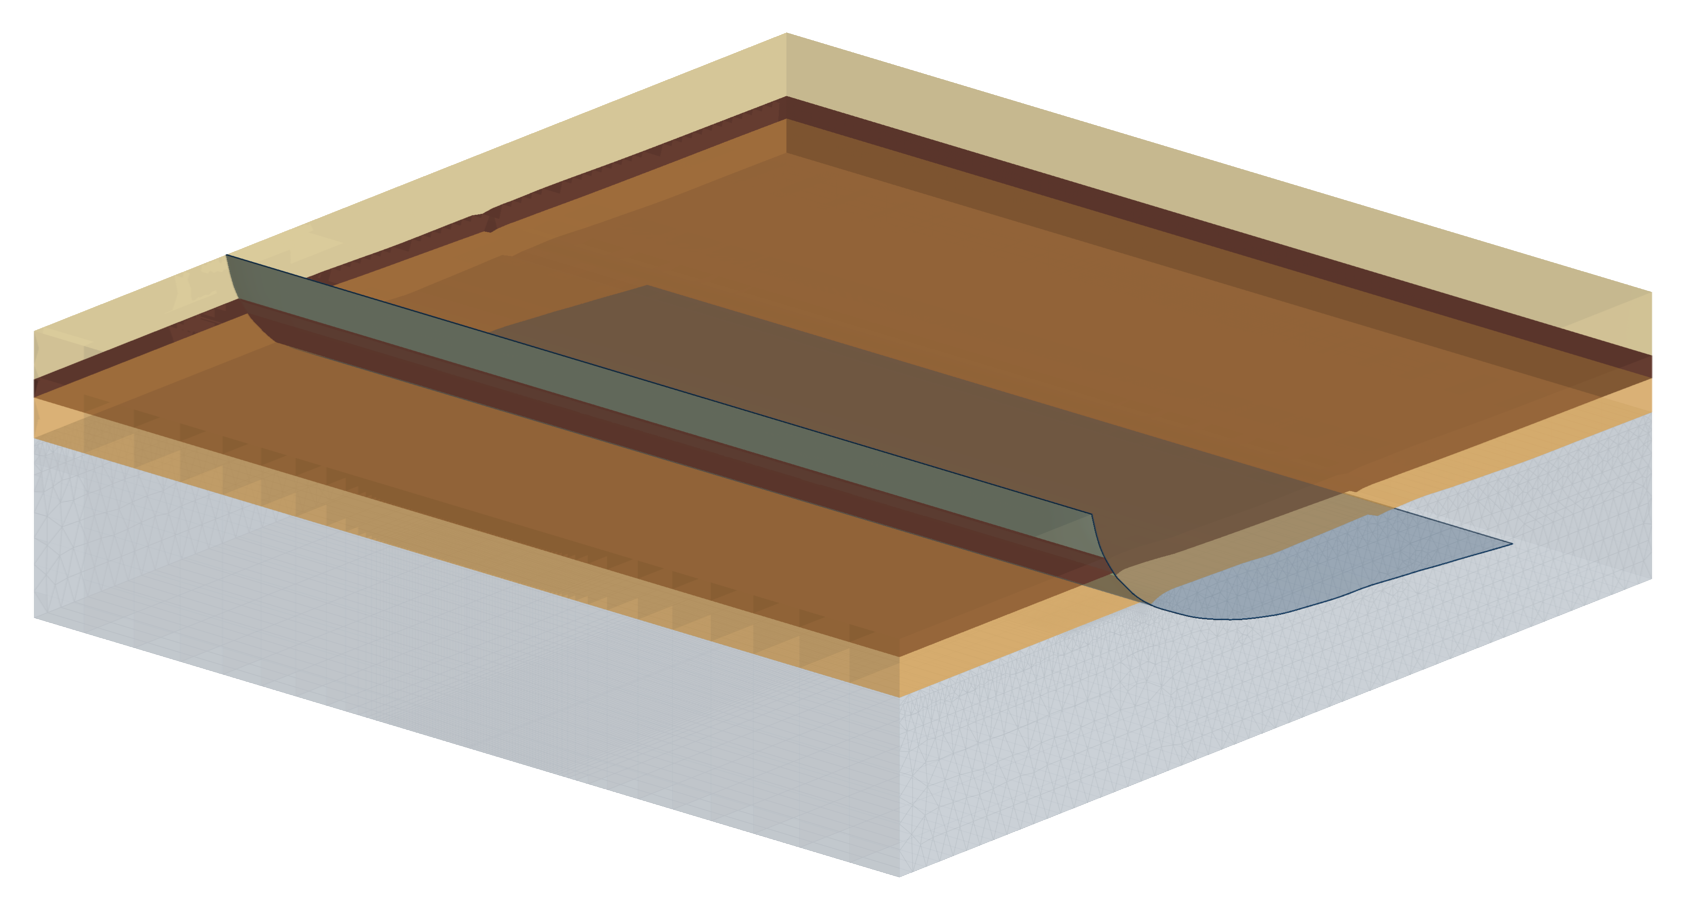
\includegraphics[
    width=32mm
  ]{assets/derived/reservoir_full_unannotated.png}};

  \workflowlegendbox{163.7}{96.0}{workflowOverburden}{Overburden}
  \workflowlegendbox{163.7}{91.4}{workflowTopSeal}{Top seal}
  \workflowlegendbox{163.7}{86.8}{workflowStorageReservoir}{Storage reservoir}
  \workflowlegendbox{163.7}{82.2}{workflowUnderburden}{Underburden}

  \fill[workflowText] (132.5,76.15) rectangle ++(1.05,1.05);
  \node[workflow left title,anchor=west] at (134.8,76.70) {CO$_2$ migration along and across the fault};

  % Workflow-only 1,000-year cross sections: Cases 6 and 7 in rows,
  % free-phase saturation and dissolved CO2 in columns with shared scales.
  \node[inner sep=0pt] at (158.5,56.7) {\includegraphics[
    width=60mm
  ]{assets/derived/panel3_migration_cross_sections_transparent.pdf}};

  \fill[workflowText] (140.0,34.7) rectangle ++(1.05,1.05);
  \node[workflow left title,anchor=west] at (142.3,35.25) {Uncertainty quantification};
  \node[workflow figure label] at (158.5,30.5) {1,620 multiphase reservoir simulations};

  % Matched workflow-only redraws of the audited migration and containment
  % diagnostics. Both assets have identical native dimensions, typography,
  % axis geometry, and transparent backgrounds.
  \node[inner sep=0pt] at (143.3,18.4) {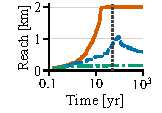
\includegraphics[
    width=27.5mm
  ]{assets/derived/panel3_uq_migration.pdf}};
  \node[workflow figure label] at (143.3,6.4) {CO$_2$ migration};

  \node[inner sep=0pt] at (173.7,18.4) {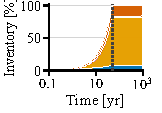
\includegraphics[
    width=27.5mm
  ]{assets/derived/panel3_uq_containment.pdf}};
  \node[workflow figure label] at (173.7,6.4) {CO$_2$ containment};

  \node[workflow figure label,align=center,text width=186mm] at (95.0,-5.2) {%
    Caption: End-to-end uncertainty quantification workflow for geologic CO$_2$ storage in faulted reservoirs.\\[-0.2pt]
    PREDICT generates stochastic local fault properties, hierarchical sampling constructs representative\\[-0.2pt]
    upscaled full-fault realizations, and JutulDarcy simulates field-scale CO$_2$ migration and containment.%
  };
\end{tikzpicture}
\end{document}
